\documentclass[12pt]{report}
\usepackage[utf8x]{inputenc}
\usepackage{graphicx}
\usepackage{textcomp, gensymb}
\usepackage{gensymb}
\usepackage{amssymb}
\usepackage{algorithm}
\usepackage[noend]{algpseudocode}
\usepackage{algpseudocode}
\graphicspath{{./images}}
\usepackage{fancyhdr}
\usepackage{blindtext}
\usepackage[colorlinks=true, urlcolor=black, linkcolor=black]{hyperref}
\hypersetup{
colorlinks=true,
linkcolor=black,
urlcolor=black
}
\usepackage{url}


\title{ETERNITY:FUNCTION F4}
\author{Tavtej Singh Lehri}
\date{}
\newcommand*{\Gtr}{\smallrel\gtr}

\makeatletter
\let\thetitle\@title
\let\theauthor\@author
\let\thedate\@date
\makeatother

\fancypagestyle{}{}
\fancyhf{}
\rhead{\thetitle}
\cfoot{\thepage}

\begin{document}

\begin{titlepage}
\centering
\vspace*{0.5 cm}

\begin{center}
\textsc{\Large CONCORDIA UNIVERSITY}\\ [2.0 cm]    
\end{center}

\textsc{\large SOEN 6011: Software Engineering Processes}\\[0.5 cm]
\rule{\linewidth}{0.2 mm}\\[0.4 cm]
{\LARGE \textbf \thetitle}\\[0.2 cm]
{\LARGE \textbf{$\Gamma$(x)}}
\rule{\linewidth}{0.2 mm}\\[1.5 cm]

\begin{center}
    {\Large \textbf{\theauthor}}\\[0.2 cm]
    {\large Student ID: 40121745}\\[2.0 cm]
    
    \begin{figure}[h!]
    \begin{center}
    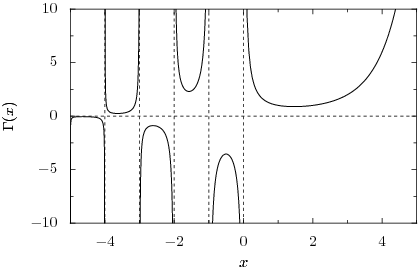
\includegraphics[width=0.5\linewidth]{Gamma_function.png}
    \end{center}
    \caption{Graph of Gamma Function.\cite{gamma}}
    \end{figure}
    
    {\large \url{https://github.com/tavtejS07/SOEN-6011}}
\end{center}

\end{titlepage}

\tableofcontents
\pagebreak

\renewcommand{\thesection}{\arabic{section}}
\section{Problem 1}
\subsection{Description}
Gamma function is said to be an extension of the factorial function used for complex numbers. For any positive integer Gamma function is defined as below.

\begin{equation}
\Gamma(x) = (x-1)\Gamma(x-1)\\
   \Rightarrow \Gamma(x) = (x-1)!
\end{equation}
\newline
\textbf{Definition: }The function which is improper integral of another function is defined as Gamma function.\cite{libretexts} Using the integral formula below we can define Gamma function. \textbf{Note: }For all positive real number x{(i.e $Re(x)>0$)}, the integral follows absolute convergence.\cite{libretexts} This was derived by \textbf{Daniel Bernoulli}.
\begin{equation}
    \Gamma(x) = \int\limits_0^\infty t^{x-1} e^{-t} dt\
\end{equation}

\subsection{Characteristics}
\begin{enumerate}
    \item $\Gamma(x)$ is defined and analytic for it's domain.\cite{libretexts}
    \item $\Gamma(x)$ displays the recursive property for $x>0$. This is displayed in equation 1 above.
    \item $\Gamma(x)$ is a meromorphic function, with $\mathbb{Z}\leq0$ as poles.\cite{gamma}
\end{enumerate}


\subsection{Domain}
Set of positive real numbers.
$x\in\mathbb{R}$ and  $x>0$
\subsection{Co-Domain}
For a specific domain, co-domain for Gamma function is
\begin{displaymath}
    \mathbb{R}>0 = \{x\in\mathbb{R}|x>0\}
\end{displaymath}

\begin{thebibliography}{9}
\addcontentsline{toc}{chapter}{Bibliography}
\bibitem{libretexts}
Libretexts. (2022, February 27). \textit{E14.2: Definition and properties of the gamma function.}Mathematics LibreTexts. Retrieved July 25, 2022, from \texttt{https://math.libretexts.org/Bookshelves/Analysis/\\Complex\_Variables\_with\_Applications\_(Orloff)/14\%3A\_Analytic\_Continuation\_\\and\_the\_Gamma\_Function/14.02\%3A\_Definition\_and\_properties\_of\_the\_Gamma\_function}

\bibitem{gamma}
Gamma function. (2011, July 25). \textit{Gamma function}- Knowino. (n.d.). Retrieved July 27, 2022, from\\ \texttt{https://www.tau.ac.il/~tsirel/dump/Static/knowino.org/wiki/Gamma\_function.html}

\end{thebibliography}

\end{document}